\documentclass[../../report.tex]{subfiles}
\graphicspath{{\subfix{../img/}}}

\begin{document}

\section{Testing Izhikevich Model}

Testing dynamics of one neuron with parameters and external input currents as described in the manuscript.

The Izhikevich model \cite{Izhikevich_2003}:
\begin{align}\label{eq_izhikevich_model}
    & \frac{dv}{dt} = \left[ 0.04v^2 + 5v + 140 - u \right] \cdot 0.05 + I + I_{syn} \\
    & \frac{du}{dt} = \left[ a (bv - u) \right] \cdot 0.05
\end{align}
where $v$ is the membrane potential, $u$ is the recovery variable, $I$ is the external current to the neuron, $I_{syn}$ is the synaptic current driven by the spikes of the presynaptic neurons. $a$ is the time scale of the recovery variable $u$, $b$ is the sensitivity of the recovery variable to sub-threshold fluctuations of the membrane potential, $c$ is the reset value of the membrane potential after spike, $d$ is the effect of slow $K^+$ and $Na^+$ conductances on the membrane potential recovery ($u$ is increased by this amount after each spike), $v_{thr}$ is the voltage threshold for spikes.

External input current is provided separately for each neuron and is given by:
\begin{equation}\label{eq_external_input_current}
    I = I_0 + \sigma \cdot N(0,1)
\end{equation}
where $I_0$ is the mean intrinsic current, $\sigma$ is the scale for the noise level, and $N(0,1)$ is the standard normal distribution with mean $0$ and variance $1$.

For R5 cells the external input current $I$ is reset after each spike. For helicon cells, $I$ is reset at each time step of the simulation ($dt=1ms$).

\begin{table}[!h]
    \centering
    \begin{tabular}{|c||c|c|c|c|c|c|c|}
        \hline
         & $a$ & $b$ & $c$ & $d$ & $I_0$ & $\sigma$ & $v_{thr}$ \\
         \hline
         \hline
        R5 during day & $0.02$ & $0.2$ & $-65$ & $6$ & $0.34$ & $0.02$ & $-10$ \\
        \hline
        R5 at night & $0.02$ & $0.3$ & $-50$ & $1.6$ & $0.3$ & $0.08$ & $-10$ \\
        \hline
        Helicon during the day & $0.02$ & $0.2$ & $-65$ & $6$ & $4.5$ & $5$ & $-10$ \\
        \hline
        Helicon during night & $0.02$ & $0.2$ & $-65$ & $6$ & $-0.75$ & $5$ & $-10$ \\
        \hline
    \end{tabular}
    \caption{Parameters of the Izhikevich model for R5 and Helicon cells at morning and night}
    \label{tab:my_label}
\end{table}

The results of the simulations are displayed in Fig. \ref{fig_example_single_helicon_r5_day_night}.

\begin{remark}
    For the simulations, the standard deviation was normalized with regard to the simulation step size ONLY for helicon cells (see Remark \ref{extended-report-remark-normalizing_std_external_current} in the extended report).
\end{remark}

\begin{note}
    
\end{note}

\begin{figure}[!hb]\label{fig_example_single_helicon_r5_day_night}
    \centering
    \subfigure[R5 during the day]{
        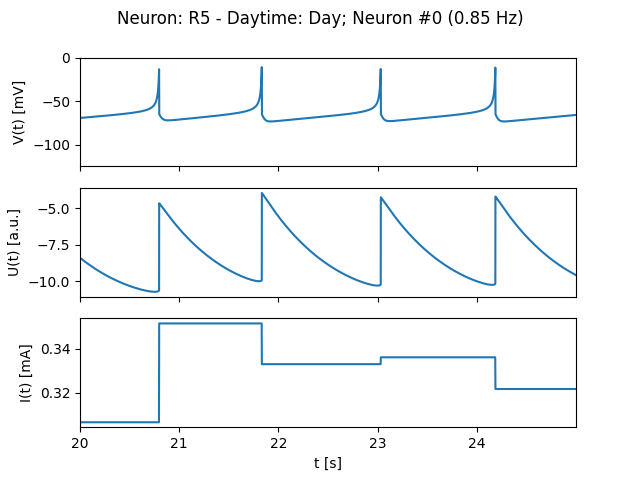
\includegraphics[width=0.45\textwidth]{img/extended_report/0_test_izhikevich/R5_Day_Neuron_0.png}
    }
    \subfigure[R5 at night]{
        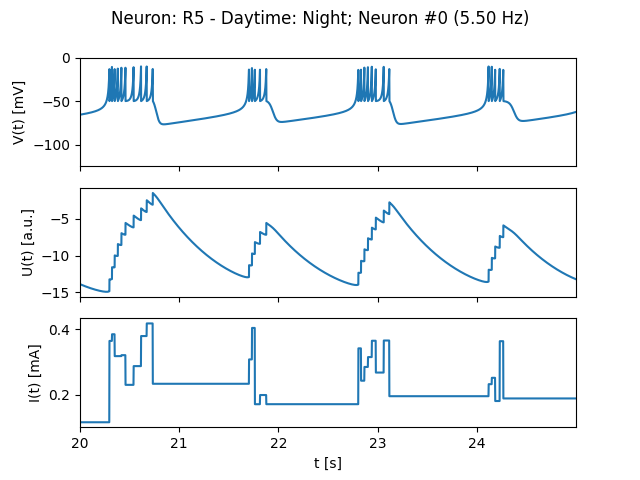
\includegraphics[width=0.45\textwidth]{img/extended_report/0_test_izhikevich/R5_Night_Neuron_0.png}
    }
    \subfigure[Helicon during the day]{
        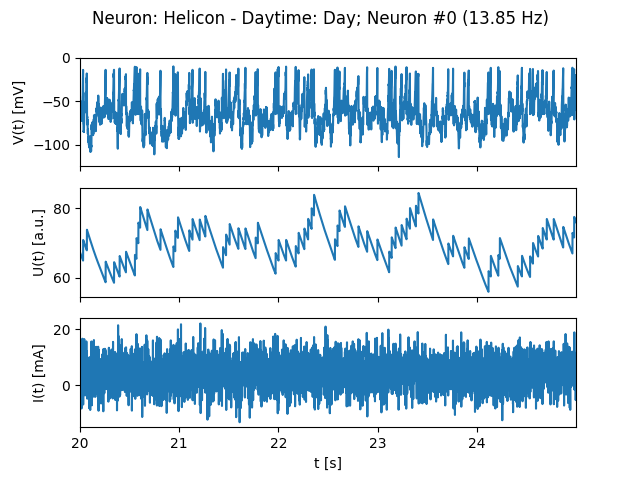
\includegraphics[width=0.45\textwidth]{img/extended_report/0_test_izhikevich/Helicon_Day_Neuron_0.png}
    }
    \subfigure[Helicon at night]{
        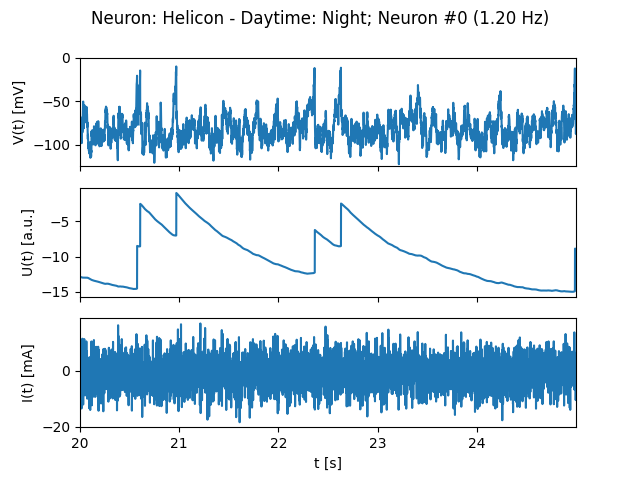
\includegraphics[width=0.45\textwidth]{img/extended_report/0_test_izhikevich/Helicon_Night_Neuron_0.png}
    }
    \caption{Comparison of R5 and Helicon at different times of day}
\end{figure}

\FloatBarrier

\end{document}